\documentclass[tikz,border=10pt]{standalone}
% https://latex.org/forum/viewtopic.php?t=27765
\usetikzlibrary{arrows,quotes}
\begin{document}
	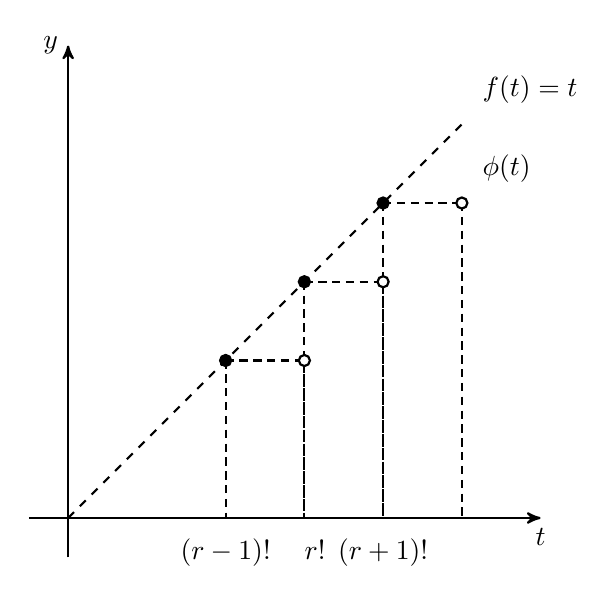
\begin{tikzpicture}[    thick,    >=stealth',     empty dot/.style = { circle, draw, fill = white!0,                          inner sep = 0pt, minimum size = 4pt },    filled dot/.style = { empty dot, fill = black}  ]  \def\r{3}  \draw[->] (-0.5,0) -- (6,0) coordinate[label = {below:$t$}] (xmax);  \draw[->] (0,-0.5) -- (0,6) coordinate[label = {left:$y$}]  (ymax);  \draw [dashed] (0,0) -- (5,5);  \foreach \i in {\r+1,\r,\r-1} {    \draw [densely dashed] (\i,\i)   -- (\i+1,\i);    \draw [densely dashed] (\i,\i)   -- (\i,0);    \draw [densely dashed] (\i+1,\i) -- (\i+1,0);    \node [filled dot] at (\i,\i) {};    \node [empty  dot] at (\i+1,\i) {};  }  \node ["above right:$f(t)=t$"]  at (5,5) {};  \node ["above right:$\phi(t)$"] at (\r+2,\r+1) {};  \node ["below:$(r-1)!$"] at (\r-1,0) {};  \node ["below:$\phantom{()}r!$"]     at (\r,0)   {};  \node ["below:$(r+1)!$"] at (\r+1,0) {};
	\end{tikzpicture}
\end{document}